\section{Método}


\begin{frame}
\frametitle{S-PTAM}
\begin{figure}[htb]
	\centering
	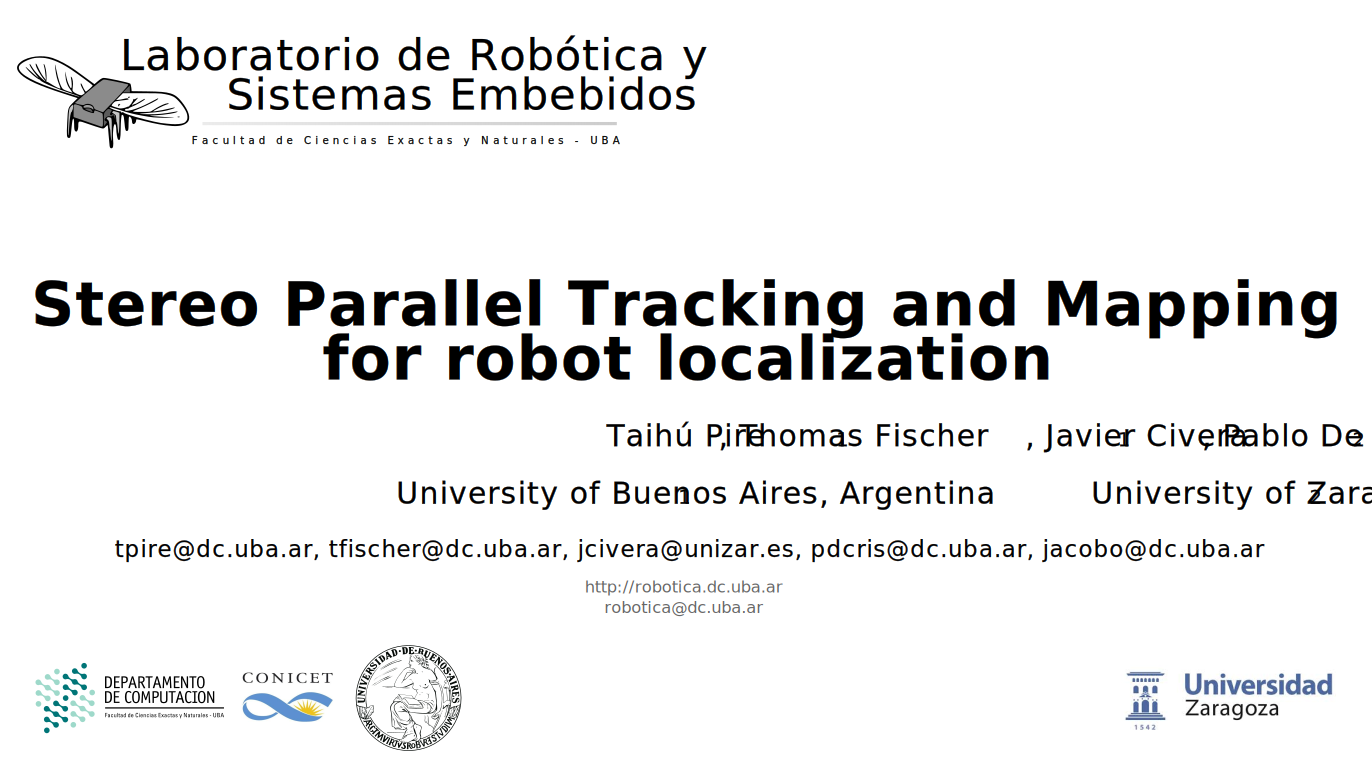
\includegraphics[width=1.0\columnwidth]{method/portada-sptam-kitti-video.pdf}
	\hfill
\end{figure}

\end{frame}


\begin{frame}
\frametitle{S-PTAM}

\begin{itemize}
\item Sistema SLAM basado en features.
\item Cámara estéreo como sensor principal.
\item Construye y mantiene un mapa disperso del entorno.
\item Basado en keyframes.
\end{itemize}

\begin{figure}[htb]
	\centering
	\includegraphics[width=0.8\columnwidth]{method/sptam_kitti.png}
\end{figure}

\end{frame}


\begin{frame}

\frametitle{Dense S-PTAM}
\begin{figure}[htb]
	\centering
	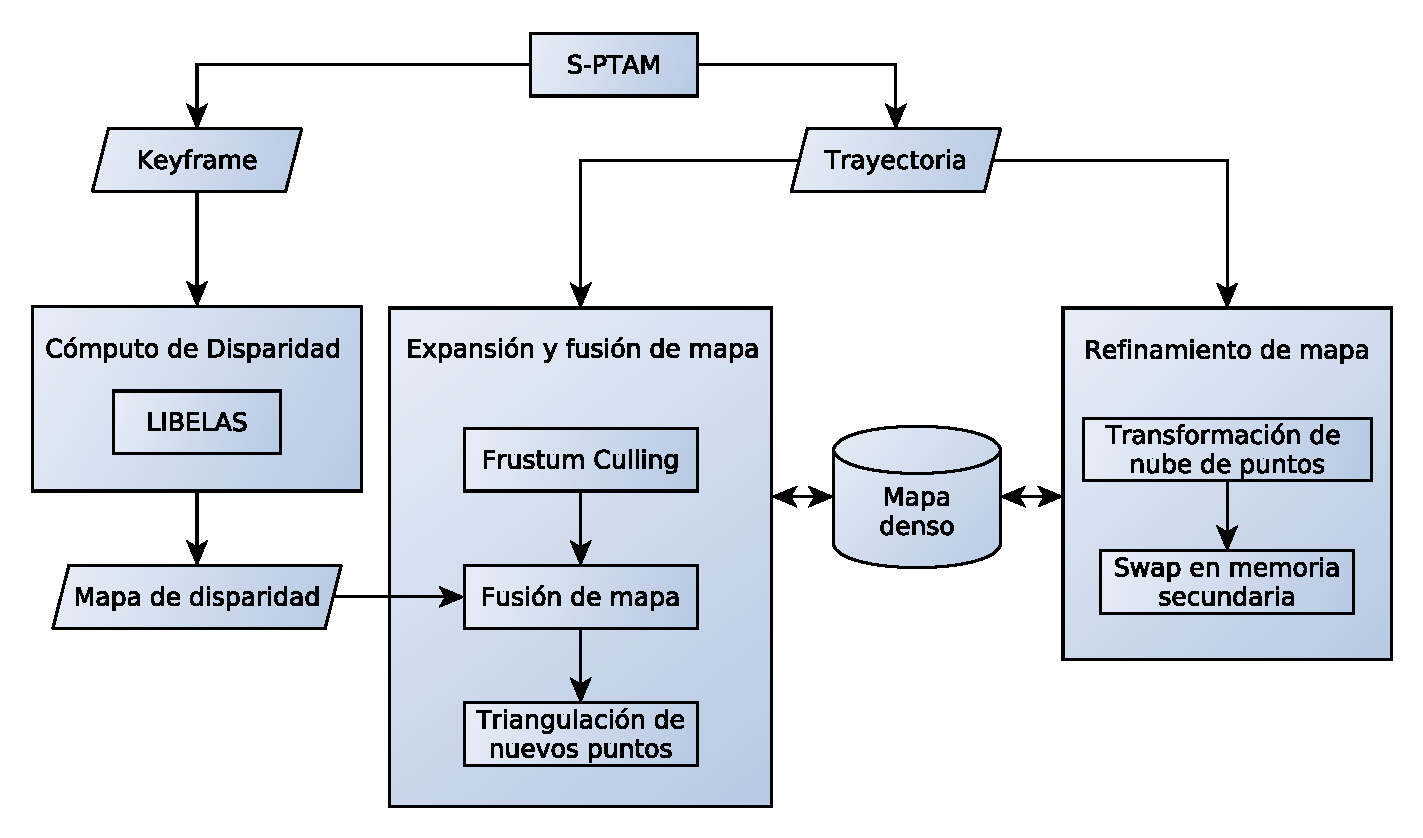
\includegraphics[width=1.0\columnwidth]{method/metodo-diagram.pdf}
	\hfill
\end{figure}

\end{frame}


\begin{frame}
\frametitle{Cómputo de disparidad}

\begin{block}{LIBELAS (Library for Efficient Large-scale Stereo Matching)}
\begin{itemize}
\item Andreas Geiger, Julius Ziegler, and Christoph Stiller. StereoScan: Dense 3d reconstruction in real-time. In \textit{2011 IEEE Intelligent Vehicles Symposium (IV)}, pages 963-968, June 2011.
\item Librería multiplataforma de código abierto para computar mapas de disparidad a partir de pares de imágenes estéreo rectificadas de alta resolución.
\end{itemize}
\end{block}

\begin{block}{Definición - Mapa de disparidad}
Función $\disparityMap:\mathbb{R}^{2}\mathbb{\rightarrow R}^{+}$ que mapea los píxeles en el plano de la imagen a su correspondiente valor de disparidad. Denominaremos $\disparityMap_{j}$ a la función que representa el mapa de disparidad generado a partir del par de imágenes estéreo del \emph{keyframe} $\keyframe_{j}$.
\end{block}

\end{frame}


\begin{frame}
\frametitle{Cómputo de disparidad}

\begin{figure}[htb]
	\centering
	\includegraphics[width=0.5\columnwidth]{method/libelas_merge_kitti04_22.jpg}
	\caption{Mapa de disparidad LIBELAS - Dataset KITTI.}
\end{figure}
\begin{figure}[htb]
	\centering
	\includegraphics[width=0.5\columnwidth]{method/libelas_merge_tsukuba_222.jpg}
	\caption{Mapa de disparidad LIBELAS - Dataset Tsukuba.}
\end{figure}

\end{frame}


\begin{frame}
	\frametitle{Expansión y fusión de mapa}
	\begin{figure}[htb]
		\centering
		\includegraphics[width=\columnwidth]{images/map_fusion.pdf}
	\end{figure}
	
	\begin{equation*}
		\point_{\mathrm{\fusion}} = \dfrac{1}{\inverseDepth_\mathrm{\fusion}} \dfrac{\point_{\mathrm{\current}}}{\norm{\point_{\mathrm{\current}}}}
		\quad \text{donde} \quad 
		\inverseDepth_{\fusion} = \dfrac{\inverseDepth_{\current} + \inverseDepth_{\previous}}{2}
	\end{equation*}
\end{frame}
